\documentclass[a4paper,12pt]{article}
\usepackage{a4wide}
\usepackage{tikz}
\usetikzlibrary{calc}
\usepackage{hyperref}
\usepackage{caption}
\usepackage{enumitem}
\usepackage{amsmath}
\usepackage[font=small,labelfont=bf]{caption}

\usepackage[ngerman]{babel}

\begin{document}

\pagenumbering{arabic}
\setlist[enumerate,1]{start=0}

\setlength{\parindent}{0em}
\section*{\noindent Blockcode}

Ihre Aufgabe ist es, das Verhalten einer Entity  namens "`blockcode"' zu programmieren. Die Entity ist in der angeh\"angten Datei "`blockcode.vhdl"' deklariert und hat folgende Eigenschaften:

\begin{itemize}
	\item Eingang: \textit{rst} vom Typ std\_logic; globaler synchroner Reset
	\item Eingang: \textit{clk} vom Typ std\_logic; globaler Takt
	\item Eingang: \textit{data\_valid} vom Typ std\_logic
	\item Eingang: \textit{data} vom Typ std\_logic\_vector mit einer L\"ange von {{DATALENGTH}}
	\item Eingang: \textit{sink\_ready} vom Typ std\_logic
	\item Ausgang: \textit{code\_valid} vom Typ std\_logic
	\item Ausgang: \textit{code} vom Typ std\_logic\_vector mit einer L\"ange von {{CODELENGTH}}

\end{itemize}

\begin{center}
\begin{tikzpicture}
\draw node [draw,rectangle, minimum height=36mm, minimum width=35mm,rounded corners=2mm,thick](entity){};

\draw[->] ($ (entity.west)+(-10mm,12.0mm)$) -- ($ (entity.west) + (0mm,12.0mm)$);
\draw[anchor=east] node at ($ (entity.west)+(-9mm,12.0mm)$){ rst };

\draw[->] ($ (entity.west)+(-10mm,6.0mm)$) -- ($ (entity.west) + (0mm,6.0mm)$);
\draw[anchor=east] node at ($ (entity.west)+(-9mm,6.0mm)$){ clk };

\draw[->] ($ (entity.west)+(-10mm,0.0mm)$) -- ($ (entity.west) + (0mm,0.0mm)$);
\draw[anchor=east] node at ($ (entity.west)+(-9mm,0.0mm)$){ data\_valid };

\draw[->] ($ (entity.west)+(-10mm,-6.0mm)$) -- ($ (entity.west) + (0mm,-6.0mm)$);
\draw[anchor=east] node at ($ (entity.west)+(-9mm,-6.0mm)$){ data };

\draw[->] ($ (entity.west)+(-10mm,-12.0mm)$) -- ($ (entity.west) + (0mm,-12.0mm)$);
\draw[anchor=east] node at ($ (entity.west)+(-9mm,-12.0mm)$){ sink\_ready };


\draw[->] ($ (entity.east) + (0mm,6.0mm)$) -- ($ (entity.east) + (10mm,6.0mm)$);
\draw[anchor=west] node at ($ (entity.east) + (9mm,6.0mm)$){ code\_valid };

\draw[->] ($ (entity.east) + (0mm,-6.0mm)$) -- ($ (entity.east) + (10mm,-6.0mm)$);
\draw[anchor=west] node at ($ (entity.east) + (9mm,-6.0mm)$){ code };


\draw node at ($ (entity) - (0,0mm)$){ blockcode };

\end{tikzpicture}
\end{center}

Ver\"andern sie die Datei "`blockcode.vhdl"' nicht!
\\

Diese Entity soll als Zwischeneinheit funktionieren, welche verschl\"usselte Blockcode Elemente aus den Daten einer Quelle \textit{source} erstellt und zu einer nachfolgenden Datensenke \textit{sink} entsprechend Abbildung~1 weiterleitet. In den folgenden Abschnitten wird n\"aher auf die \"Ubertragung und die Verschl\"usselung eingegangen.
\\

\begin{figure}[h!]
\centering
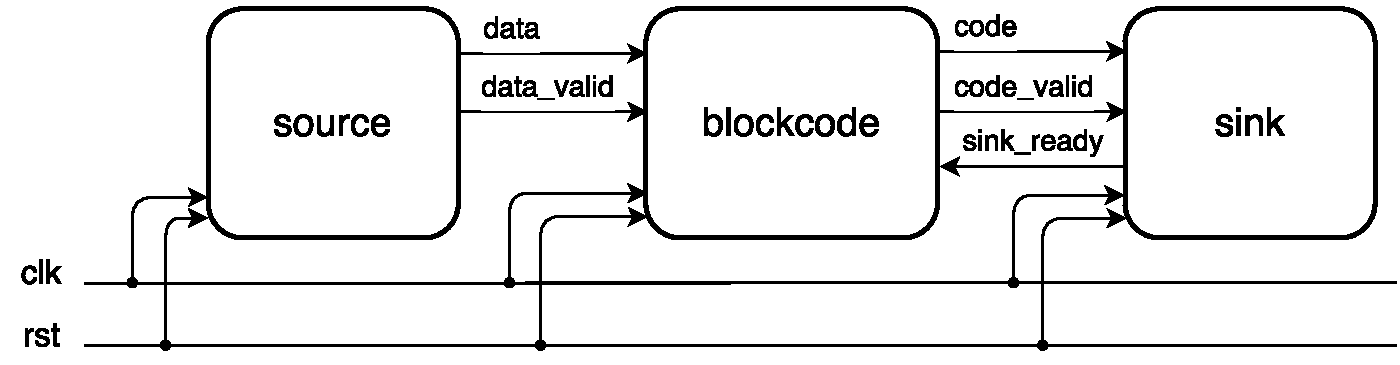
\includegraphics[scale=0.6]{../static/system_view.pdf}
\caption{Systemansicht. Die Quelle \textit{source} erzeugt Daten, welche von der Entity verschl\"usselt und anschlie"send an die nachfolgende Datensenke \textit{sink} weitergeleitet werden.}
\end{figure}

\newpage
\subsection*{\noindent \"Ubertragung}

\textbf{\"Ubertragung der Daten von "`source"' $\rightarrow$ "`blockcode"':} Folgende Ports sind hierf\"ur relevant:
\begin{itemize}
\item \textbf{data:} Enth\"alt die Daten, welche als Blockcode verschl\"usselt werden sollen.
\item \textbf{valid\_data:} Zeigt an, ob die Daten am Port \textit{data} in diesem Taktzyklus g\"ultig sind. Die "`blockcode"' Entity soll nur g\"ultige Daten verschl\"usseln.
\end{itemize}

\textbf{\"Ubertragung der Daten von "`blockcode"' $\rightarrow$ "`sink"':} Dies ist eine Verbindung mit R\"uckmeldung, bei der die Senke angiebt, wann sie bereit zum Empfangen von Daten ist. Folgende Ports sind hierf\"ur relevant:
\begin{itemize}
\item \textbf{code:} Enth\"alt den verschl\"usselten Code, welcher aus g\"ultigen Daten des Ports \textit{data} erzeugt wurde.
\item \textbf{code\_valid:} Gibt an, ob der Code am Port \textit{code}  in diesem Taktzyklus g\"ultig ist.
\item \textbf{sink\_ready:} Gibt an, ob die Senke bereit zum Empfangen eines Codes ist.
\end{itemize}

\textbf{R\"uckmeldung:} Wenn die Senke nicht bereit zum Empfangen ist, wird der Port \textit{sink\_ready} auf '0' gesetzt. Die Entity "`blockcode"' soll den selben Code solange senden, bis die Senke bereit ist. Die Senke erfasst einen Code nur dann, wenn beide Ports \textit{code\_valid} und \textit{sink\_ready} gesetzt (= '1') sind.\\
\\
\textbf{Buffering:} Da die Senke die \"Ubertragung verz\"ogern kann, wird innerhalb der Entity "`blockcode"' ein Buffer ben\"otig (z.B. zirkul\"arer FIFO). F\"ur diese Aufgabe soll Ihr Buffer maximal 4 Elemente zwischenspeichern k\"onnen. \\
\\
\textbf{Synchrone Ausg\"ange:} Alle Ausg\"ange der Entities in diesem System sind an den gemeinsamen Takt \textit{clk} gebunden. Ver\"anderungen an diesen Ports sollen daher nur bei einer steigenden Flanke des Taktsignals \textit{clk} geschehen.\\

\newpage
\subsection*{\noindent Verschl\"usselung}

Das Datenwort soll als $[{{CODELENGTH}},{{DATALENGTH}}]$ Blockcode verschl\"usselt werden. Dies bedeutet, dass die {{DATALENGTH}} Datenbits mit {{NUMPARITY}} Parit\"atsbits erg\"anzt werden:

\begin{equation}
d = (d_0,d_1, .. d_{{LASTDATAELEM}}) \longrightarrow c = (d_0,d_1,...,d_{{LASTDATAELEM}},p_0,...,p_{{LASTPARITYELEM}})
\end{equation}

Die Verschl\"usselung erfolgt mit Hilfe der Generator-Matrix G:

\begin{equation}
c = d \cdot G
\end{equation}

Verwenden Sie die gegebene Generator-Matrix, welche aus einer Einheitsmatrix und der Parit\"ats-Matrix besteht (getrennt durch die vertikale Linie):

\begin{center}
\[
\left(
\begin{array}{ {{MATRIXHEADER}} }
{{GENERATORMATRIX}}
\end{array}
\right)
\]
\end{center}

\textbf{Tipp:} Da ein + im Bin\"arsystem gleich dem XOR ist, k\"onnen sie die Parit\"at mittels XOR berechnen. \\
\\

\textbf{Beispiel einer Verschl\"usselung:} ({{EXAMPLEDATA}}) $\longrightarrow$ ({{EXAMPLECODE}}) \\

\newpage
\subsection*{\noindent Systemverhalten}

\begin{figure}[h!]
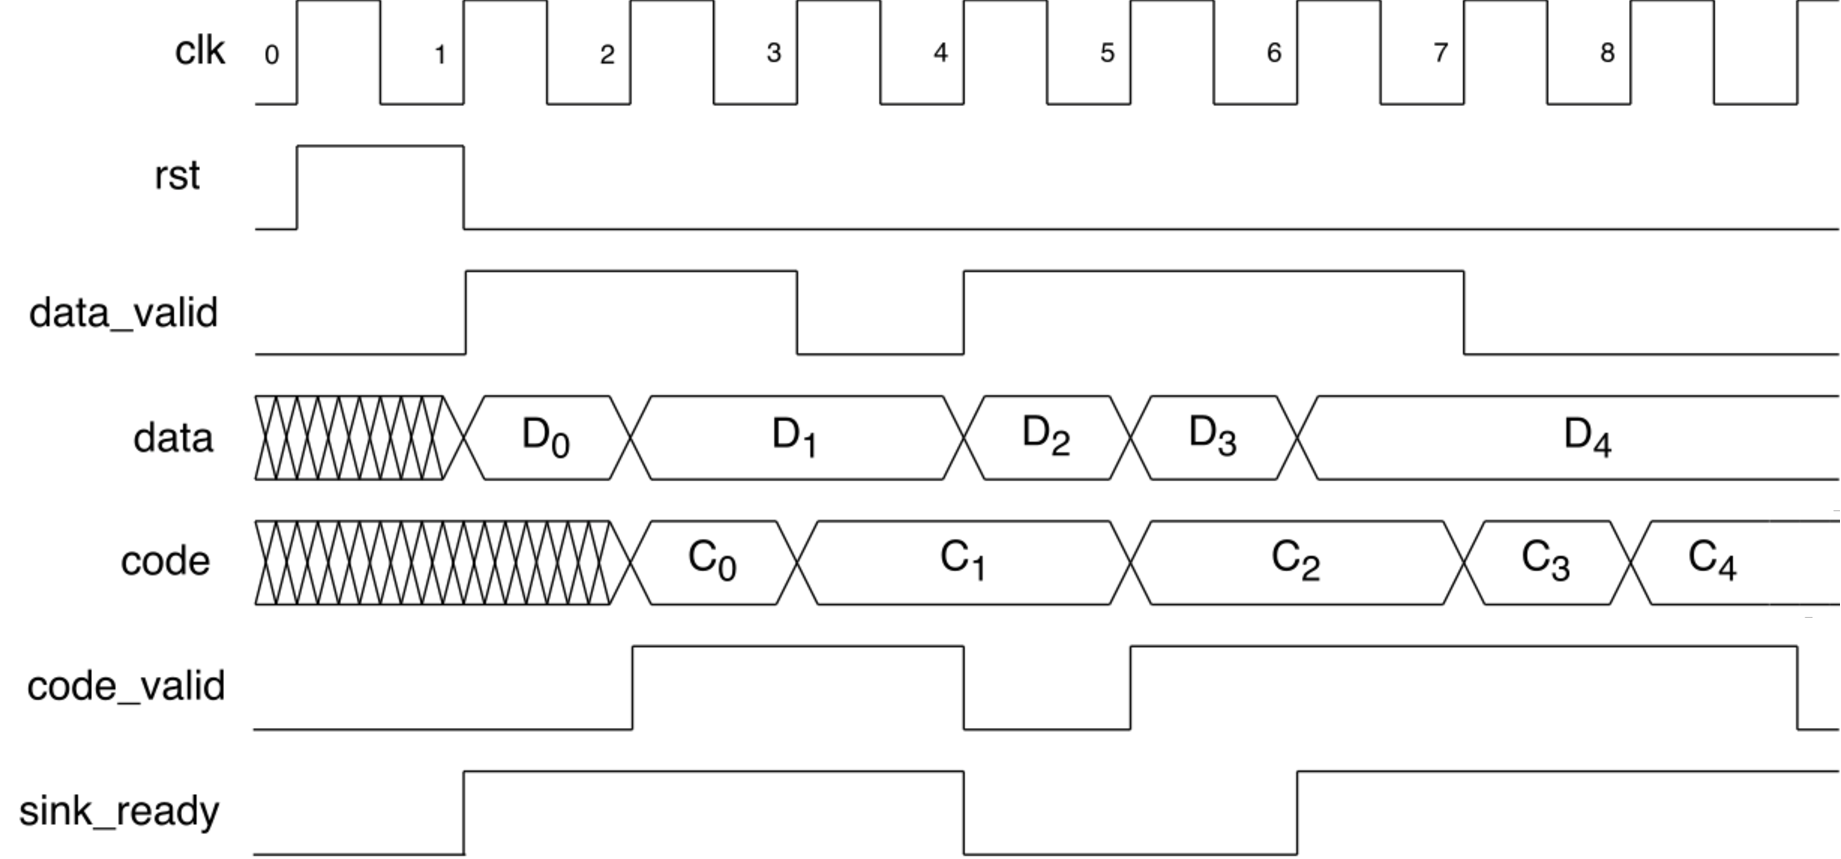
\includegraphics[scale=0.5]{../static/diagram.pdf}

\caption{Beispielhaftes Verhalten des Systems. Die Zahlen entsprechen dem Start des jeweiligen Taktzyklus.}
\end{figure}

Abbildung~2 veranschaulicht beispielhaft das geforderte Verhalten der Entity "`blockcode"' f\"ur die einzelnen Taktzyklen:
\begin{enumerate}
\item Globaler Reset.
\item Ein g\"ultiges Datenelement $D_0$ ist gegeben. Dies ist dadurch gekennzeichnet, dass \textit{data\_valid} gesetzt ist.
\item Ein neues g\"ultiges Datenelement $D_1$ ist gegeben. Das verschl\"usselte Element $C_0$ wird f\"ur die \"Ubertragung gesetzt. Die Senke ist bereit zum Empfang, was an dem gesetzten Port \textit{sink\_ready} erkennbar ist, und erfasst daher das Code Element $C_0$ in diesem Taktzyklus.
\item Es ist kein g\"ultiges Datenelement gegeben, da \textit{data\_valid} nicht gesetzt ist. Das verschl\"usselte Element $C_1$ wird \"ubertragen und von der Senke erfasst.
\item Ein neues g\"ultiges Datenelement $D_2$ ist gegeben. Da $C_1$ bereits erfasst wurde, muss es nicht erneut gesetzt werden und es findet keine \"Ubertragung statt. Daher ist \textit{code\_valid} auch nicht gesetzt.
\item Ein neues g\"ultiges Datenelement $D_3$ ist gegeben. Das verschl\"usselte Element $C_2$ wird f\"ur die \"Ubertragung gesetzt. Da \textit{sink\_ready} nicht gesetzt ist, ist die Senke jedoch nicht f\"ur den Empfang bereit.
\item Ein neues g\"ultiges Datenelement $D_4$ ist gegeben. Da $C_2$ im letzten Takt nicht erfasst wurde, bleibt es gesetzt. Die Senke ist nun wieder bereit und erfasst $C_2$.
\item Kein neues g\"ultiges Datenelement ist gegeben. $C_3$ wird gesetzt und erfasst.
\item Kein neues g\"ultiges Datenelement ist gegeben. $C_4$ wird gesetzt und erfasst.
\end{enumerate}

\vspace{0.7cm}

Programmieren Sie dieses Verhalten in der angeh\"angten Datei "`blockcode\_beh.vhdl"'.\\

Um Ihre L\"osung abzugeben, senden Sie ein E-Mail mit dem Betreff "`Result Task {{ TASKNR }}"' und Ihrer Datei "`blockcode\_beh.vhdl"'  an {{ SUBMISSIONEMAIL }}.

\vspace{0.7cm}

Viel Erfolg und m\"oge die Macht mit Ihnen sein.

\end{document}
